\section{Problem Statement}  \label{RSS:sec:problem}

In this section, we formally define the form of data augmentation studied in this paper. We define a dataset $\dataset$ as a list of examples $\example\in\exampleSpace$ and, optionally, labels $\ell(\example)=\classLabel$, where $\ell$ is a task-specific labeling function. We assume the space $\exampleSpace$ is a metric space with a distance function $\distfname$. Augmentation is a stochastic function $\augDef$ which takes in an example $\example$ and produces the augmented example $\exampleAug$. The general form is shown in Algorithm \ref{RSS:alg:aug_prototype}. Internally, augmentation will call \sample{} to generate a vector of parameters, which we call $\transform$. We also define $\exampleAugSet$ as a set of $k$ augmented examples produced by calling \sample{} then \apply{} $k$ times. The parameters $\transform$ describe the transformation which will be applied to the example in the \apply{} procedure. We focus on augmentation functions that are stochastic, thus $\augf$ will sample new augmented examples each time it is called. If the dataset contains labels $\classLabel$, we assume that the labels should not change when the example is augmented.

\begin{algorithm}[t]
\caption{$\augf(x)$}\label{RSS:alg:aug_prototype}
$\transform = \sample{}(\example) $\\
$\aug{\example} = \apply(\example,\transform)$\\
return $\aug{\example}$\\
\end{algorithm}

We propose that useful augmentations should be \textit{valid}, \textit{relevant}, and \textit{diverse}. Let the valid set $\validSet$ be the set of examples which are physically possible. Let the relevant set $\relevantSet$ be the set of examples likely to occur when collecting data for or executing a specific set of tasks in a specific domain. We define $\mathrm{validity}(\exampleAug)=1$ if $\exampleAug \in \validSet$ and $\mathrm{validity}(\exampleAug)=0$ otherwise. We also define $\mathrm{relevance}(\exampleAug):=e^{-\distf{\exampleAug}{\relevantSet}}$ and $\mathrm{diversity}(\exampleAugSet):=\uniformity$, where $\klF$ is the Kullback–Leibler divergence and $\transformDist$ is the distribution of the parameters for a set of augmented examples $\exampleAugSet$. Diversity is maximized when the augmentation transformations are uniformly distributed in the range $\transformUniformRange$. With these concepts defined, we define data augmentation as the following optimization problem, the solution to which is a set of augmentations $\exampleAugSet$:

\begin{equation}
    \label{RSS:eq:most_general}
    \begin{array}{cc}
        \underset{\exampleAugSet}{\mathrm{max}} & \mathrm{diversity}(\exampleAugSet) + \beta \sum_{\exampleAug_i}\mathrm{relevance}(\exampleAug_i) \\
        \mathrm{subject\: to} & \mathrm{validity}(\exampleAug_i)\:\:\quad \forall\,\exampleAug_i \in \exampleAugSet\\
        & \ell(\aug{\example})=\ell(\example) \\
    \end{array}
\end{equation}

\noindent where $\beta$ is a positive scalar.

This optimization problem can be solved directly if $\validSet$, $\relevantSet$, and $\ell$ are known. However, in manipulation tasks, that is rarely the case. Instead, we will formulate an approximation to this problem using measures of relevance, diversity, and validity that are derived from physics and useful for a variety of robotic manipulation tasks and domains.

\begin{figure}
    \centering
    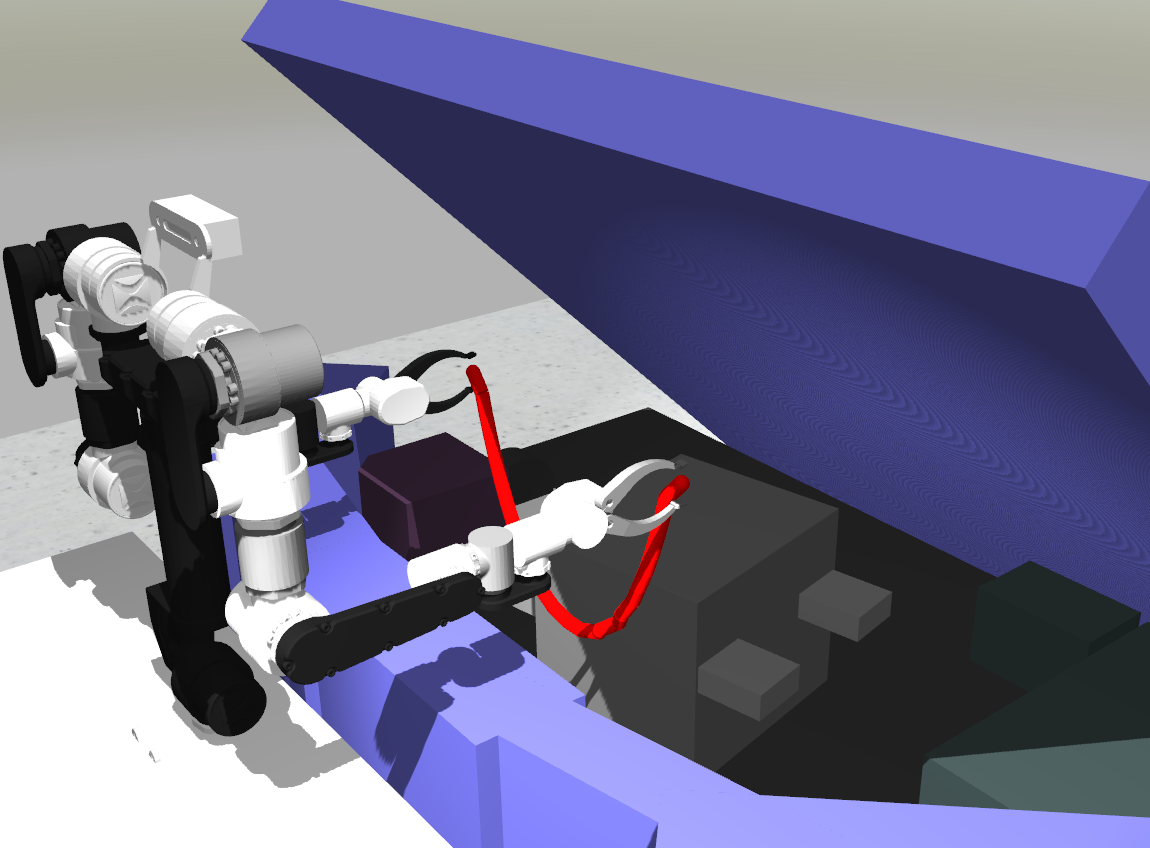
\includegraphics[height=5cm]{Chap3/images/car_sim_env-cropped.png}
    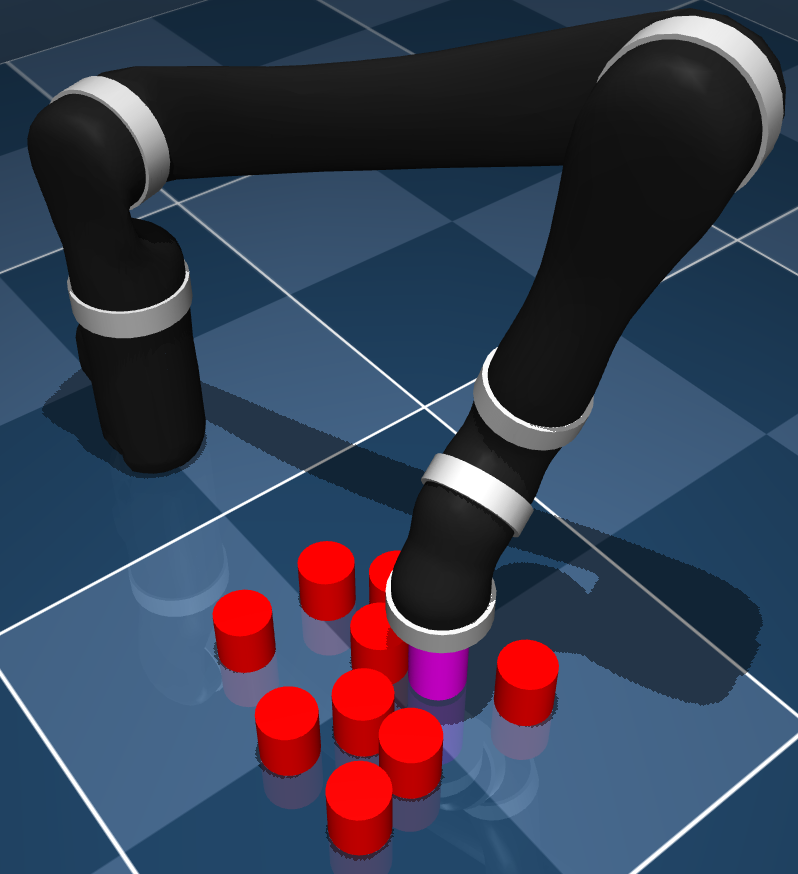
\includegraphics[height=5cm]{Chap3/images/cylinders_env.png}
    \caption{(left) The environment for bimanual rope manipulation, in simulation. (right) The environment for cluttered planar pushing of cylinders, in simulation.}
    \label{RSS:fig:sim_envs}
\end{figure}

\subsection{Assumptions}
\label{RSS:sec:assumptions}

Most augmentation algorithms rely on some expert knowledge or heuristics to define what is a valid augmentation. For instance, rotating an image for image classification makes an assumption that rotation does not change the label, and this is not always true. Similarly, the efficacy or correctness of our algorithm is also subject to certain assumptions. Here, we define the key assumptions:

\begin{itemize}
    \item The geometry of the robot and all objects is known.
    \item The scene can be decomposed into objects which can be assigned or detected as either moving or stationary.
    \item Examples are time-series, consisting of at least two states.
    \item All possible contacts between stationary vs. moving objects have the same friction coefficient.
    \item Contacts between the robot and objects/environment (e.g. grasps) can be determined from the data.
    \item A rigid-body transformation of an object preserves internal forces arising from its material properties.
    \item Objects only move due to contact or under the force of gravity. We do not handle movement due to magnetism or wind, for example.
\end{itemize}

Notably, the assumption that a rigid-body transformation preserves internal, material forces is what allows us to handle cluttered scenes with many moving objects, as well as deformable or articulated objects. While it could be valuable to augment the deformation or relative motion of the objects, doing so in a way that is valid would be challenging. Instead, we transform them all rigidly (See examples in Figures \ref{RSS:fig:rope_aug_examples},\ref{RSS:fig:cylinders_aug_examples}).

The assumption of having a common friction coefficient between all moving versus stationary objects is in-line with much manipulation research. For example, work on planar pushing assumes friction is uniform across the plane \cite{PushSim2021,PushYu2016}. Note that we make no assumption on the coefficients of friction between two moving objects.

Naturally, there are scenarios where these assumptions do not hold and thus where our algorithm may not perform well. However, our experiments demonstrate significant improvement on two very different manipulation scenarios, and we expect these assumptions extend to other scenarios as well.